\documentclass[]{article}
\usepackage{lmodern}
\usepackage{amssymb,amsmath}
\usepackage{ifxetex,ifluatex}
\usepackage{fixltx2e} % provides \textsubscript
\ifnum 0\ifxetex 1\fi\ifluatex 1\fi=0 % if pdftex
  \usepackage[T1]{fontenc}
  \usepackage[utf8]{inputenc}
\else % if luatex or xelatex
  \ifxetex
    \usepackage{mathspec}
  \else
    \usepackage{fontspec}
  \fi
  \defaultfontfeatures{Ligatures=TeX,Scale=MatchLowercase}
\fi
% use upquote if available, for straight quotes in verbatim environments
\IfFileExists{upquote.sty}{\usepackage{upquote}}{}
% use microtype if available
\IfFileExists{microtype.sty}{%
\usepackage{microtype}
\UseMicrotypeSet[protrusion]{basicmath} % disable protrusion for tt fonts
}{}
\usepackage[margin=1in]{geometry}
\usepackage{hyperref}
\hypersetup{unicode=true,
            pdftitle={Heterogeneity- Subgroup Analysis and Meta-Regression},
            pdfauthor={Michail Belias},
            pdfborder={0 0 0},
            breaklinks=true}
\urlstyle{same}  % don't use monospace font for urls
\usepackage{color}
\usepackage{fancyvrb}
\newcommand{\VerbBar}{|}
\newcommand{\VERB}{\Verb[commandchars=\\\{\}]}
\DefineVerbatimEnvironment{Highlighting}{Verbatim}{commandchars=\\\{\}}
% Add ',fontsize=\small' for more characters per line
\usepackage{framed}
\definecolor{shadecolor}{RGB}{248,248,248}
\newenvironment{Shaded}{\begin{snugshade}}{\end{snugshade}}
\newcommand{\AlertTok}[1]{\textcolor[rgb]{0.94,0.16,0.16}{#1}}
\newcommand{\AnnotationTok}[1]{\textcolor[rgb]{0.56,0.35,0.01}{\textbf{\textit{#1}}}}
\newcommand{\AttributeTok}[1]{\textcolor[rgb]{0.77,0.63,0.00}{#1}}
\newcommand{\BaseNTok}[1]{\textcolor[rgb]{0.00,0.00,0.81}{#1}}
\newcommand{\BuiltInTok}[1]{#1}
\newcommand{\CharTok}[1]{\textcolor[rgb]{0.31,0.60,0.02}{#1}}
\newcommand{\CommentTok}[1]{\textcolor[rgb]{0.56,0.35,0.01}{\textit{#1}}}
\newcommand{\CommentVarTok}[1]{\textcolor[rgb]{0.56,0.35,0.01}{\textbf{\textit{#1}}}}
\newcommand{\ConstantTok}[1]{\textcolor[rgb]{0.00,0.00,0.00}{#1}}
\newcommand{\ControlFlowTok}[1]{\textcolor[rgb]{0.13,0.29,0.53}{\textbf{#1}}}
\newcommand{\DataTypeTok}[1]{\textcolor[rgb]{0.13,0.29,0.53}{#1}}
\newcommand{\DecValTok}[1]{\textcolor[rgb]{0.00,0.00,0.81}{#1}}
\newcommand{\DocumentationTok}[1]{\textcolor[rgb]{0.56,0.35,0.01}{\textbf{\textit{#1}}}}
\newcommand{\ErrorTok}[1]{\textcolor[rgb]{0.64,0.00,0.00}{\textbf{#1}}}
\newcommand{\ExtensionTok}[1]{#1}
\newcommand{\FloatTok}[1]{\textcolor[rgb]{0.00,0.00,0.81}{#1}}
\newcommand{\FunctionTok}[1]{\textcolor[rgb]{0.00,0.00,0.00}{#1}}
\newcommand{\ImportTok}[1]{#1}
\newcommand{\InformationTok}[1]{\textcolor[rgb]{0.56,0.35,0.01}{\textbf{\textit{#1}}}}
\newcommand{\KeywordTok}[1]{\textcolor[rgb]{0.13,0.29,0.53}{\textbf{#1}}}
\newcommand{\NormalTok}[1]{#1}
\newcommand{\OperatorTok}[1]{\textcolor[rgb]{0.81,0.36,0.00}{\textbf{#1}}}
\newcommand{\OtherTok}[1]{\textcolor[rgb]{0.56,0.35,0.01}{#1}}
\newcommand{\PreprocessorTok}[1]{\textcolor[rgb]{0.56,0.35,0.01}{\textit{#1}}}
\newcommand{\RegionMarkerTok}[1]{#1}
\newcommand{\SpecialCharTok}[1]{\textcolor[rgb]{0.00,0.00,0.00}{#1}}
\newcommand{\SpecialStringTok}[1]{\textcolor[rgb]{0.31,0.60,0.02}{#1}}
\newcommand{\StringTok}[1]{\textcolor[rgb]{0.31,0.60,0.02}{#1}}
\newcommand{\VariableTok}[1]{\textcolor[rgb]{0.00,0.00,0.00}{#1}}
\newcommand{\VerbatimStringTok}[1]{\textcolor[rgb]{0.31,0.60,0.02}{#1}}
\newcommand{\WarningTok}[1]{\textcolor[rgb]{0.56,0.35,0.01}{\textbf{\textit{#1}}}}
\usepackage{graphicx,grffile}
\makeatletter
\def\maxwidth{\ifdim\Gin@nat@width>\linewidth\linewidth\else\Gin@nat@width\fi}
\def\maxheight{\ifdim\Gin@nat@height>\textheight\textheight\else\Gin@nat@height\fi}
\makeatother
% Scale images if necessary, so that they will not overflow the page
% margins by default, and it is still possible to overwrite the defaults
% using explicit options in \includegraphics[width, height, ...]{}
\setkeys{Gin}{width=\maxwidth,height=\maxheight,keepaspectratio}
\IfFileExists{parskip.sty}{%
\usepackage{parskip}
}{% else
\setlength{\parindent}{0pt}
\setlength{\parskip}{6pt plus 2pt minus 1pt}
}
\setlength{\emergencystretch}{3em}  % prevent overfull lines
\providecommand{\tightlist}{%
  \setlength{\itemsep}{0pt}\setlength{\parskip}{0pt}}
\setcounter{secnumdepth}{0}
% Redefines (sub)paragraphs to behave more like sections
\ifx\paragraph\undefined\else
\let\oldparagraph\paragraph
\renewcommand{\paragraph}[1]{\oldparagraph{#1}\mbox{}}
\fi
\ifx\subparagraph\undefined\else
\let\oldsubparagraph\subparagraph
\renewcommand{\subparagraph}[1]{\oldsubparagraph{#1}\mbox{}}
\fi

%%% Use protect on footnotes to avoid problems with footnotes in titles
\let\rmarkdownfootnote\footnote%
\def\footnote{\protect\rmarkdownfootnote}

%%% Change title format to be more compact
\usepackage{titling}

% Create subtitle command for use in maketitle
\newcommand{\subtitle}[1]{
  \posttitle{
    \begin{center}\large#1\end{center}
    }
}

\setlength{\droptitle}{-2em}

  \title{Heterogeneity- Subgroup Analysis and Meta-Regression}
    \pretitle{\vspace{\droptitle}\centering\huge}
  \posttitle{\par}
    \author{Michail Belias}
    \preauthor{\centering\large\emph}
  \postauthor{\par}
      \predate{\centering\large\emph}
  \postdate{\par}
    \date{12 February 2019}


\begin{document}
\maketitle

\hypertarget{introduction}{%
\section{Introduction}\label{introduction}}

Bassler et.al (Bassler et al. 2004) conducted a Cochrane Review to
evaluate the effects of Ketotifen alone or in combination with other
co-interventions in children with asthma and/or wheezing. The primary
outcome was the use of rescue bronchodilators. In the systematic review,
a random effects model with the risk ratio as measure of treatment
effect was used throughout. The meta-analysis of the clinical judgement
data contains 10 trials.

Let's import the data in to start our analysis. In order to do that we
have to call the \emph{readxl} package using the library(``readxl'')
command. If a package is not installed in your computer you can install
by using the \emph{install.packages(`name of the package')} command

\begin{Shaded}
\begin{Highlighting}[]
\KeywordTok{library}\NormalTok{(}\StringTok{"readxl"}\NormalTok{)}
\NormalTok{Ketotifen =}\StringTok{  }\KeywordTok{read_xlsx}\NormalTok{(}\StringTok{"Data/Ketotifen.xlsx"}\NormalTok{)}
\end{Highlighting}
\end{Shaded}

We can see the first rows of our data with the \emph{head()} command.

\begin{Shaded}
\begin{Highlighting}[]
\KeywordTok{head}\NormalTok{(Ketotifen, }
     \DataTypeTok{n =}\DecValTok{10} \CommentTok{# number of row we want to print}
\NormalTok{     )}
\end{Highlighting}
\end{Shaded}

\begin{verbatim}
# A tibble: 10 x 6
   study            Ee    Ne    Ec    Nc blind  
   <chr>         <dbl> <dbl> <dbl> <dbl> <chr>  
 1 Chay              1    10     6    10 Blinded
 2 Rackam           31    68    38    65 Blinded
 3 Van Asperen      16    52    19    51 Blinded
 4 Croce            19    39    17    36 unclear
 5 de Benedictis     7    34    35    41 unclear
 6 Longo            10    18    15    18 unclear
 7 Montoya           6    20    14    20 unclear
 8 Mulhern           6    16     8    15 unclear
 9 Salmon            8    28    16    34 unclear
10 Spicak            9    25    20    25 unclear
\end{verbatim}

Our assumption is that the treatment effects come from a distribution
rather than from a common effect. We want to generalise our conclusions
to broader populations, therefore we will perform a random-effect model.
We will use the \emph{meta} package. The primary function for
dichotomous outcomes is \emph{metabin()}

\begin{Shaded}
\begin{Highlighting}[]
\KeywordTok{library}\NormalTok{(}\StringTok{"meta"}\NormalTok{)}
\end{Highlighting}
\end{Shaded}

\textbf{Reminder: An easy way to check the help file of any package
and/or functions is to use the \emph{?} or \emph{??} and then the name
of the function or package, for instance \emph{??metabin}.} \emph{meta}
package has an excellent help file, take advantage of it.

\newline 

\newline  \newline

\newline 

In your computer please fill the \ldots{} , in the metabin command with
the appropriate variables from the data. We want to perform a
random-effects meta-analysis with risk ratio as an effect size measure,
using the empirical Bayes (EB) as a \(\tau^2\) estimator.

\begin{Shaded}
\begin{Highlighting}[]
\NormalTok{res.RE =}\StringTok{ }\KeywordTok{metabin}\NormalTok{(}\DataTypeTok{event.e =}\NormalTok{ .. ,      }\CommentTok{## Events of treated}
                 \DataTypeTok{n.e =}\NormalTok{ .. ,          }\CommentTok{## Total number of treated}
                 \DataTypeTok{event.c =}\NormalTok{ .. ,      }\CommentTok{## Events of control}
                 \DataTypeTok{n.c =}\NormalTok{ ..,           }\CommentTok{## Total number of treated}
                 \DataTypeTok{sm =}\NormalTok{ ..,            }\CommentTok{## Effect size}
                 \DataTypeTok{method =}\NormalTok{ ..,        }\CommentTok{## weight calculation method}
                 \DataTypeTok{data =}\NormalTok{ ..,          }\CommentTok{## the data-set}
                 \DataTypeTok{studlab =}\NormalTok{ ..,       }\CommentTok{## The trial names}
                 \DataTypeTok{method.tau=}\NormalTok{..,      }\CommentTok{## tau estimator method}
                 \DataTypeTok{comb.fixed =}\NormalTok{...,    }\CommentTok{## A logical (TRUE/FALSE) indicating whether a fixed or random  }
                 \DataTypeTok{comb.random=}\NormalTok{...     }\CommentTok{## effect meta-analysis should be conducted.}
\NormalTok{                 )}
\end{Highlighting}
\end{Shaded}

Print the output and make a forest plot out of them. Also show the
p-value of the overall treatment effect (\textbf{Hint:
test.overall.random = TRUE})

\textbf{What is the Inverse-Variance method? Are there any other
choices? If yes which?}

\newline 

\newline 

\newline 

\textbf{Interpret the results}

\newline 

\newline 

\newline 

\newline 

\newline 

\newline 

\textbf{Does the Ketotifen help the patients?} \textbf{How much is the
increase/decrease of the use of rescue bronchodilators ?} \newline 

\newline 

\newline 

\newline 

\newline 

\newline 

\textbf{Describe what Q , \(I^2\) , \(tau^2\) and H are and then report
their estimated values}

\newline 

\newline 

\newline 

\newline 

\newline 

\newline 

\textbf{Do our data agree with the random-effects model assumption?}

\newline 

\newline 

\newline 

\newline 

\newline 

\newline 

\textbf{Is the heterogeneity large?}

\newline 

\newline 

\newline 

\newline 

\newline 

\newline 

\newpage

\hypertarget{subgroup-analysis}{%
\subsection{Subgroup analysis}\label{subgroup-analysis}}

\emph{Until now we 1) did a systematic review, 2) gathered the Ketotifen
data, 3) conducted a meta-analysis, in order to find out whether the use
of Ketotifen is beneficial or not and 4) we pooled our treatment effects
using a random-effects model, because we assumed that the treatment
effects of the trials come from a distribution.}

This is one aim of meta-analysis. Another is to investigate our data in
order to understand where do these between-study differences come from.
We observed, that some trials had a common design. Particularly Chay et
al., Rackham et al., and Van Asperen et al.~used blinding. We wonder if
we can explain some heterogeneity, by splitting the trials into two
meta-analyses. One for the blinded and one for not-blinded trials.

\textbf{Blinding is a trial characteristic, not a patient
characteristic, therefore we can perform subgroup analysis. If the
categorical variable was a patient characteristic, for instance gender
then we should NOT split the trial and then perform a subgroup analysis.
We will discuss this case later on}

TIn order to perform a subgroup analysis we use again the function
\textbf{metabin()}, but adding also the option \textbf{byvar = ``name of
the subgrouping variable''}.

\begin{Shaded}
\begin{Highlighting}[]
\NormalTok{res.SA =}\StringTok{ }\KeywordTok{metabin}\NormalTok{(}\DataTypeTok{event.e =}\NormalTok{ .. ,      }\CommentTok{## Events of treated}
                 \DataTypeTok{n.e =}\NormalTok{ .. ,          }\CommentTok{## Total number of treated}
                 \DataTypeTok{event.c =}\NormalTok{ .. ,      }\CommentTok{## Events of control}
                 \DataTypeTok{n.c =}\NormalTok{ ..,           }\CommentTok{## Total number of treated}
                 \DataTypeTok{sm =}\NormalTok{ ..,            }\CommentTok{## Effect size}
                 \DataTypeTok{method =}\NormalTok{ ..,        }\CommentTok{## weight calculation method}
                 \DataTypeTok{data =}\NormalTok{ ..,          }\CommentTok{## the data-set}
                 \DataTypeTok{studlab =}\NormalTok{ ..,       }\CommentTok{## The trial names}
                 \DataTypeTok{method.tau=}\NormalTok{..,      }\CommentTok{## tau estimator method}
                 \DataTypeTok{comb.fixed =}\NormalTok{...,    }\CommentTok{## A logical (TRUE/FALSE) indicating whether a fixed or random  }
                 \DataTypeTok{comb.random=}\NormalTok{...,    }\CommentTok{## effect meta-analysis should be conducted.}
                 \DataTypeTok{byvar =}\NormalTok{ ...         }\CommentTok{## The splitting variable  }
\NormalTok{                 )}
\end{Highlighting}
\end{Shaded}

Print the output and make a forest plot out of them. Also show the
p-value of the overall treatment effect (\textbf{Hint:
test.overall.random = TRUE})

\textbf{Note: for better looking forest-plots see the help file (
??forest.meta )}

The subgroup analysis shows that method of blinding does not explain
adequately the statistical heterogeneity between trials. \emph{Why?}

\textbf{Report the results for subgroups (random effects model) table
(copy-paste)}

\newline 

\newline 

\textbf{What are the values of \(Q_{per subgroup}\), \(I^2\) , H and
\(tau^2\) now? What do they represent?}

\newline 

\newline 

\newline 

\newline 

\newline 

\textbf{Report the Test for subgroup differences (copy-paste). How
should you interpret it? Discuss Q, d.f. and p-value.}

\newline 

\newline 

\newline 

\newline 

\newline 

\newpage

Subgroup analysis has a lot in common with a meta-regression with a
categorical independent variable. We can also perform a subgroup
analysis in a ``linear'' meta-regression framework. Particularly, we can
use the \emph{metareg()} function to fit a meta-regression, using the
log risk ratios as a dependent variable and the blinding as an
independent one. The options need a \emph{meta} object (the random
effects meta-analysis we performed earlier is one) and the categorical
variable we wish to use (in our case blinding).

\textbf{Fill the \ldots{}.}

\begin{Shaded}
\begin{Highlighting}[]
\NormalTok{res.MR.SA =}\KeywordTok{metareg}\NormalTok{(}\DataTypeTok{x =}\NormalTok{ .... , }\CommentTok{## an object of class meta}
                  \DataTypeTok{formula =}\NormalTok{ ....,}
                  \DataTypeTok{hakn =}\NormalTok{ T)}
\end{Highlighting}
\end{Shaded}

Compare the subgroup analysis with the meta-regression output. There
some minor differences, but this is due the fact that the \(\tau^2\)
within the blinded and unclear groups are different in subgroup
analysis, while in meta-regression they are the same. If in the subgroup
analysis we ``force'' the \(\tau^2\)s for both subgroups to be equal,
then the results of the meta-regression are exactly the same as Subgroup
analysis.

\begin{Shaded}
\begin{Highlighting}[]
\NormalTok{res.SA}\FloatTok{.2}\NormalTok{ =}\StringTok{ }\KeywordTok{metabin}\NormalTok{(}\DataTypeTok{event.e =}\NormalTok{ Ee ,      }\CommentTok{## Events of treated}
                 \DataTypeTok{n.e =}\NormalTok{ Ne ,          }\CommentTok{## Total number of treated}
                 \DataTypeTok{event.c =}\NormalTok{ Ec ,      }\CommentTok{## Events of control}
                 \DataTypeTok{n.c =}\NormalTok{ Nc,           }\CommentTok{## Total number of treated}
                 \DataTypeTok{sm =} \StringTok{"RR"}\NormalTok{,          }\CommentTok{## Effect size}
                 \DataTypeTok{method =} \StringTok{"Inverse"}\NormalTok{, }\CommentTok{## weight calculation method}
                 \DataTypeTok{data =}\NormalTok{ Ketotifen,   }\CommentTok{## the data-set}
                 \DataTypeTok{studlab =}\NormalTok{ study,    }\CommentTok{## The trial names}
                 \DataTypeTok{method.tau=}\StringTok{"EB"}\NormalTok{,    }\CommentTok{## tau estimator method}
                 \DataTypeTok{byvar =}\NormalTok{  blind,     }\CommentTok{## The splitting variable  }
                 \DataTypeTok{comb.fixed =}\NormalTok{ F,    }\CommentTok{## A logical variable (True/False) indicating }
                                     \CommentTok{## whether a fixed effect meta-analysis should be conducted.}
                 \DataTypeTok{tau.common =}\NormalTok{ T}
\NormalTok{                 )}

\CommentTok{# forest(res.SA)}
\end{Highlighting}
\end{Shaded}

\hypertarget{meta-regression-with-a-continuous-covariate}{%
\subsection{Meta-regression with a continuous
covariate}\label{meta-regression-with-a-continuous-covariate}}

In this section we will try to explain again part of the heterogeneity,
but instead of using a categorical variable we will use a continuous.

We will use the meta-analysis of Colditz et al.~(Colditz 1994), where he
evaluated the overall effectiveness of the Bacillus Calmette-Guerin
vaccine against tuberculosis. In addition, covariates that may
potentially influence the effect of vaccination were examined.

\textbf{Note: we using AGAIN a variable that is a trial characteristic,
not a patient characteristic}

\begin{Shaded}
\begin{Highlighting}[]
\KeywordTok{library}\NormalTok{(metafor)}
\NormalTok{dat <-}\StringTok{ }\NormalTok{dat.colditz1994}
\KeywordTok{head}\NormalTok{(dat)}
\end{Highlighting}
\end{Shaded}

\begin{verbatim}
  trial               author year tpos  tneg cpos  cneg ablat     alloc
1     1              Aronson 1948    4   119   11   128    44    random
2     2     Ferguson & Simes 1949    6   300   29   274    55    random
3     3      Rosenthal et al 1960    3   228   11   209    42    random
4     4    Hart & Sutherland 1977   62 13536  248 12619    52    random
5     5 Frimodt-Moller et al 1973   33  5036   47  5761    13 alternate
6     6      Stein & Aronson 1953  180  1361  372  1079    44 alternate
\end{verbatim}

We believe that part of our data heterogeneity can be due to the
country's place on the world map. That is a resonable thing in epidemic,
since the climate may affect the disease. Therefore, we will fit a
meta-regression using the logRR as dependent variable and he absolute
geographical latitude.

First, perform a random-effects meta-analysis and then fit a
meta-regression using the absolute geographical latitude (``ablat'') as
a moderator.

\begin{Shaded}
\begin{Highlighting}[]
\NormalTok{res.RE.MR =}\KeywordTok{metareg}\NormalTok{(}\DataTypeTok{x =}\NormalTok{ .... , }\CommentTok{## an object of class meta}
                  \DataTypeTok{formula =}\NormalTok{ ....,}
                  \DataTypeTok{hakn =}\NormalTok{ T)}
\end{Highlighting}
\end{Shaded}

\textbf{Report the Test for Residual Heterogeneity and the Test for
Moderators}

\newline 

\newline 

\newline 

\newline 

\newline 

\textbf{What are our conclusions?}

\newline 

\newline 

\newline 

\newline 

\newline 

We can also plot the effect estimates over the range of the absolute
geographical latitude, so that we may have a visual represantion, using
the \emph{bubble()} command. See the help file
(\emph{??bubble.metareg}).

\begin{Shaded}
\begin{Highlighting}[]
\KeywordTok{bubble}\NormalTok{(res.RE.MR)}
\end{Highlighting}
\end{Shaded}

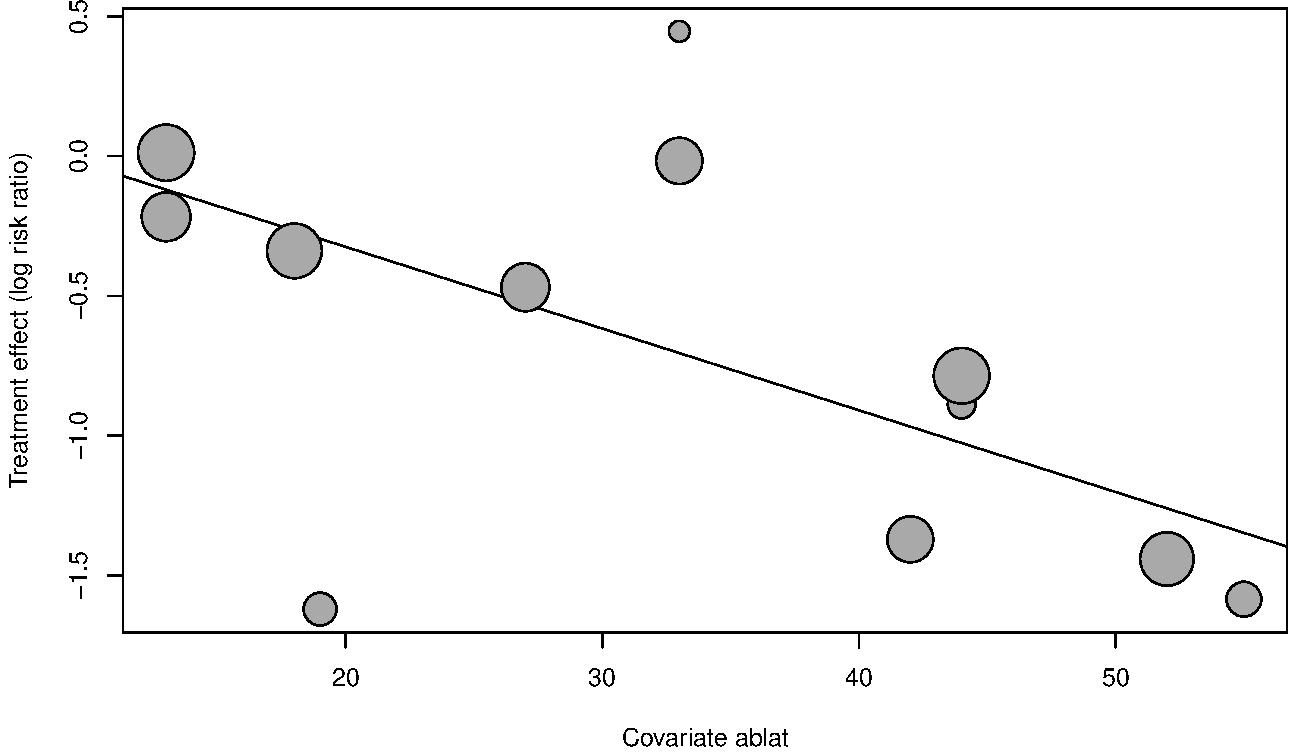
\includegraphics{Figs/unnamed-chunk-16-1.pdf}

\textbf{Based on our model calculate the predicted logRR (and then RR)
for Nijmegen (or any other city you like)}

\newline 

\newline 

\newline 

\newline 

\newline 

\textbf{What are the absolute geographical latitude ranges we can safely
predict?}

\newline 

\newline 

\newline 

\newline 

\newline 

\newpage

\hypertarget{references}{%
\section*{References}\label{references}}
\addcontentsline{toc}{section}{References}

\hypertarget{refs}{}
\leavevmode\hypertarget{ref-Bassler_2004}{}%
Bassler, Dirk, Andrew AD Mitra, Francine M Ducharme, Johannes Forster,
and Guido Schwarzer. 2004. ``Ketotifen Alone or as Additional Medication
for Long-Term Control of Asthma and Wheeze in Children.'' \emph{Cochrane
Database of Systematic Reviews}, January.
\url{https://doi.org/10.1002/14651858.cd001384.pub2}.

\leavevmode\hypertarget{ref-Colditz_1994}{}%
Colditz, Graham A. 1994. ``Efficacy of BCG Vaccine in the Prevention of
Tuberculosis.'' \emph{JAMA} 271 (9): 698.
\url{https://doi.org/10.1001/jama.1994.03510330076038}.


\end{document}
